% Graphic for TeX using PGF
% Title: /home/guillaume/Documents/Université de Montréal/Automne 2014/Génie logiciel/Devoir/devoir-3/diagramme-de-classes-changement-1.dia
% Creator: Dia v0.97.3
% CreationDate: Sun Dec  7 16:12:28 2014
% For: guillaume
% \usepackage{tikz}
% The following commands are not supported in PSTricks at present
% We define them conditionally, so when they are implemented,
% this pgf file will use them.
\ifx\du\undefined
  \newlength{\du}
\fi
\setlength{\du}{15\unitlength}
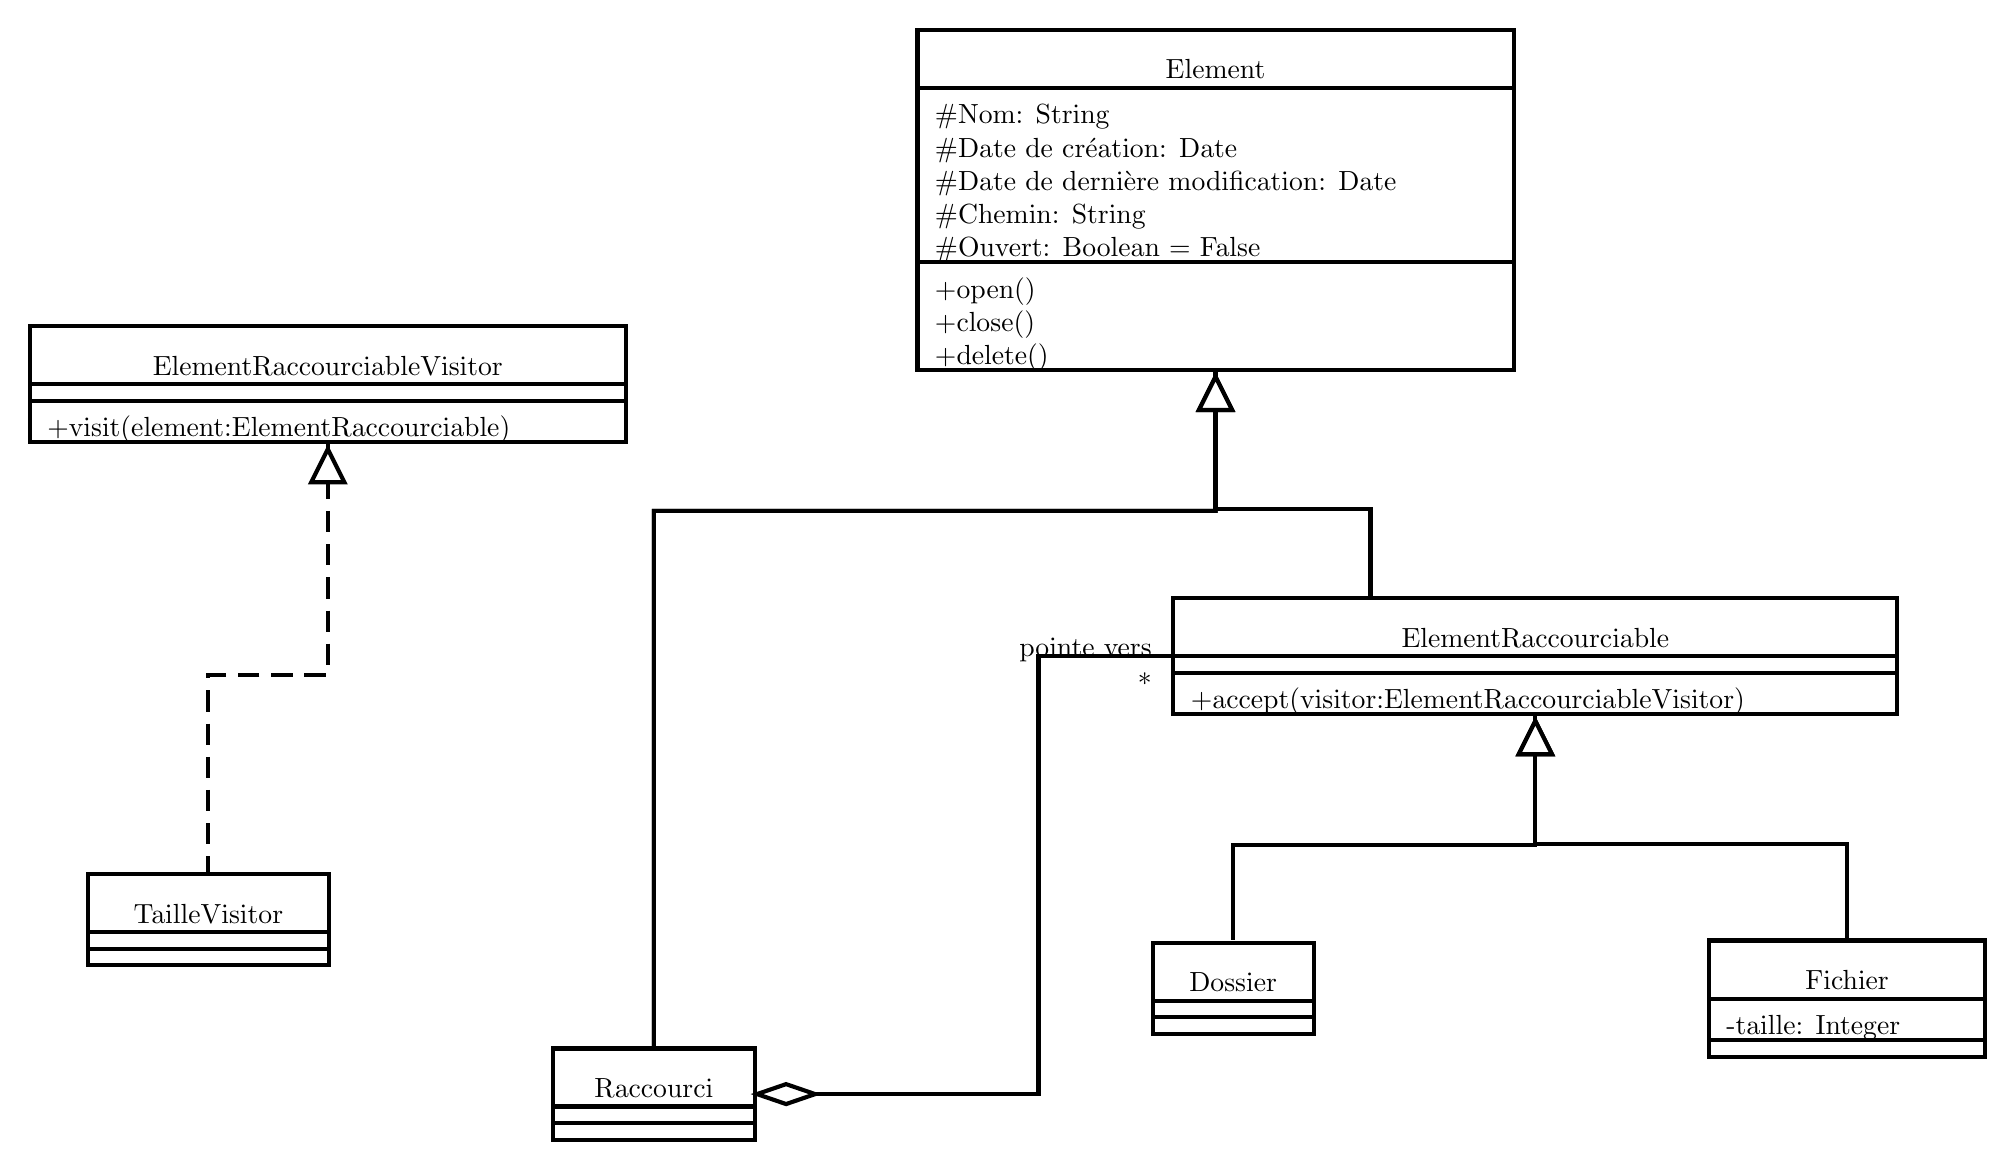
\begin{tikzpicture}
\pgftransformxscale{1.000000}
\pgftransformyscale{-1.000000}
\definecolor{dialinecolor}{rgb}{0.000000, 0.000000, 0.000000}
\pgfsetstrokecolor{dialinecolor}
\definecolor{dialinecolor}{rgb}{1.000000, 1.000000, 1.000000}
\pgfsetfillcolor{dialinecolor}
\pgfsetlinewidth{0.100000\du}
\pgfsetdash{}{0pt}
\definecolor{dialinecolor}{rgb}{1.000000, 1.000000, 1.000000}
\pgfsetfillcolor{dialinecolor}
\fill (16.600000\du,18.800000\du)--(16.600000\du,20.200000\du)--(21.470000\du,20.200000\du)--(21.470000\du,18.800000\du)--cycle;
\definecolor{dialinecolor}{rgb}{0.000000, 0.000000, 0.000000}
\pgfsetstrokecolor{dialinecolor}
\draw (16.600000\du,18.800000\du)--(16.600000\du,20.200000\du)--(21.470000\du,20.200000\du)--(21.470000\du,18.800000\du)--cycle;
% setfont left to latex
\definecolor{dialinecolor}{rgb}{0.000000, 0.000000, 0.000000}
\pgfsetstrokecolor{dialinecolor}
\node at (19.035000\du,19.750000\du){Raccourci};
\definecolor{dialinecolor}{rgb}{1.000000, 1.000000, 1.000000}
\pgfsetfillcolor{dialinecolor}
\fill (16.600000\du,20.200000\du)--(16.600000\du,20.600000\du)--(21.470000\du,20.600000\du)--(21.470000\du,20.200000\du)--cycle;
\definecolor{dialinecolor}{rgb}{0.000000, 0.000000, 0.000000}
\pgfsetstrokecolor{dialinecolor}
\draw (16.600000\du,20.200000\du)--(16.600000\du,20.600000\du)--(21.470000\du,20.600000\du)--(21.470000\du,20.200000\du)--cycle;
\definecolor{dialinecolor}{rgb}{1.000000, 1.000000, 1.000000}
\pgfsetfillcolor{dialinecolor}
\fill (16.600000\du,20.600000\du)--(16.600000\du,21.000000\du)--(21.470000\du,21.000000\du)--(21.470000\du,20.600000\du)--cycle;
\definecolor{dialinecolor}{rgb}{0.000000, 0.000000, 0.000000}
\pgfsetstrokecolor{dialinecolor}
\draw (16.600000\du,20.600000\du)--(16.600000\du,21.000000\du)--(21.470000\du,21.000000\du)--(21.470000\du,20.600000\du)--cycle;
\pgfsetlinewidth{0.100000\du}
\pgfsetdash{}{0pt}
\pgfsetmiterjoin
\pgfsetbuttcap
{
\definecolor{dialinecolor}{rgb}{0.000000, 0.000000, 0.000000}
\pgfsetfillcolor{dialinecolor}
% was here!!!
\definecolor{dialinecolor}{rgb}{0.000000, 0.000000, 0.000000}
\pgfsetstrokecolor{dialinecolor}
\draw (21.519766\du,19.900000\du)--(28.300000\du,19.900000\du)--(28.300000\du,9.350000\du)--(31.501449\du,9.350000\du);
}
\definecolor{dialinecolor}{rgb}{0.000000, 0.000000, 0.000000}
\pgfsetstrokecolor{dialinecolor}
\draw (22.778345\du,19.900000\du)--(28.300000\du,19.900000\du)--(28.300000\du,9.350000\du)--(31.501449\du,9.350000\du);
\pgfsetdash{}{0pt}
\pgfsetmiterjoin
\pgfsetbuttcap
\definecolor{dialinecolor}{rgb}{1.000000, 1.000000, 1.000000}
\pgfsetfillcolor{dialinecolor}
\fill (21.519766\du,19.900000\du)--(22.219766\du,19.660000\du)--(22.919766\du,19.900000\du)--(22.219766\du,20.140000\du)--cycle;
\pgfsetlinewidth{0.100000\du}
\pgfsetdash{}{0pt}
\pgfsetmiterjoin
\pgfsetbuttcap
\definecolor{dialinecolor}{rgb}{0.000000, 0.000000, 0.000000}
\pgfsetstrokecolor{dialinecolor}
\draw (21.519766\du,19.900000\du)--(22.219766\du,19.660000\du)--(22.919766\du,19.900000\du)--(22.219766\du,20.140000\du)--cycle;
% setfont left to latex
\definecolor{dialinecolor}{rgb}{0.000000, 0.000000, 0.000000}
\pgfsetstrokecolor{dialinecolor}
\node[anchor=west] at (28.400000\du,14.475000\du){};
\definecolor{dialinecolor}{rgb}{0.000000, 0.000000, 0.000000}
\pgfsetstrokecolor{dialinecolor}
\node[anchor=west] at (23.119766\du,19.750000\du){};
\definecolor{dialinecolor}{rgb}{0.000000, 0.000000, 0.000000}
\pgfsetstrokecolor{dialinecolor}
\node[anchor=east] at (31.301449\du,9.200000\du){ pointe vers};
\definecolor{dialinecolor}{rgb}{0.000000, 0.000000, 0.000000}
\pgfsetstrokecolor{dialinecolor}
\node[anchor=east] at (31.301449\du,10.000000\du){*};
\pgfsetlinewidth{0.100000\du}
\pgfsetdash{}{0pt}
\pgfsetmiterjoin
\pgfsetbuttcap
{
\definecolor{dialinecolor}{rgb}{0.000000, 0.000000, 0.000000}
\pgfsetfillcolor{dialinecolor}
% was here!!!
\definecolor{dialinecolor}{rgb}{0.000000, 0.000000, 0.000000}
\pgfsetstrokecolor{dialinecolor}
\draw (32.565000\du,2.509124\du)--(32.565000\du,5.850000\du)--(19.034877\du,5.850000\du)--(19.034990\du,18.750034\du);
}
\definecolor{dialinecolor}{rgb}{0.000000, 0.000000, 0.000000}
\pgfsetstrokecolor{dialinecolor}
\draw (32.565000\du,3.420927\du)--(32.565000\du,5.850000\du)--(19.034877\du,5.850000\du)--(19.034990\du,18.750034\du);
\pgfsetmiterjoin
\definecolor{dialinecolor}{rgb}{1.000000, 1.000000, 1.000000}
\pgfsetfillcolor{dialinecolor}
\fill (32.965000\du,3.420927\du)--(32.565000\du,2.620927\du)--(32.165000\du,3.420927\du)--cycle;
\pgfsetlinewidth{0.100000\du}
\pgfsetdash{}{0pt}
\pgfsetmiterjoin
\definecolor{dialinecolor}{rgb}{0.000000, 0.000000, 0.000000}
\pgfsetstrokecolor{dialinecolor}
\draw (32.965000\du,3.420927\du)--(32.565000\du,2.620927\du)--(32.165000\du,3.420927\du)--cycle;
% setfont left to latex
\pgfsetlinewidth{0.100000\du}
\pgfsetdash{}{0pt}
\definecolor{dialinecolor}{rgb}{1.000000, 1.000000, 1.000000}
\pgfsetfillcolor{dialinecolor}
\fill (31.550000\du,7.950000\du)--(31.550000\du,9.350000\du)--(48.990000\du,9.350000\du)--(48.990000\du,7.950000\du)--cycle;
\definecolor{dialinecolor}{rgb}{0.000000, 0.000000, 0.000000}
\pgfsetstrokecolor{dialinecolor}
\draw (31.550000\du,7.950000\du)--(31.550000\du,9.350000\du)--(48.990000\du,9.350000\du)--(48.990000\du,7.950000\du)--cycle;
% setfont left to latex
\definecolor{dialinecolor}{rgb}{0.000000, 0.000000, 0.000000}
\pgfsetstrokecolor{dialinecolor}
\node at (40.270000\du,8.900000\du){ElementRaccourciable};
\definecolor{dialinecolor}{rgb}{1.000000, 1.000000, 1.000000}
\pgfsetfillcolor{dialinecolor}
\fill (31.550000\du,9.350000\du)--(31.550000\du,9.750000\du)--(48.990000\du,9.750000\du)--(48.990000\du,9.350000\du)--cycle;
\definecolor{dialinecolor}{rgb}{0.000000, 0.000000, 0.000000}
\pgfsetstrokecolor{dialinecolor}
\draw (31.550000\du,9.350000\du)--(31.550000\du,9.750000\du)--(48.990000\du,9.750000\du)--(48.990000\du,9.350000\du)--cycle;
\definecolor{dialinecolor}{rgb}{1.000000, 1.000000, 1.000000}
\pgfsetfillcolor{dialinecolor}
\fill (31.550000\du,9.750000\du)--(31.550000\du,10.750000\du)--(48.990000\du,10.750000\du)--(48.990000\du,9.750000\du)--cycle;
\definecolor{dialinecolor}{rgb}{0.000000, 0.000000, 0.000000}
\pgfsetstrokecolor{dialinecolor}
\draw (31.550000\du,9.750000\du)--(31.550000\du,10.750000\du)--(48.990000\du,10.750000\du)--(48.990000\du,9.750000\du)--cycle;
% setfont left to latex
\definecolor{dialinecolor}{rgb}{0.000000, 0.000000, 0.000000}
\pgfsetstrokecolor{dialinecolor}
\node[anchor=west] at (31.700000\du,10.450000\du){+accept(visitor:ElementRaccourciableVisitor)};
\pgfsetlinewidth{0.100000\du}
\pgfsetdash{}{0pt}
\definecolor{dialinecolor}{rgb}{1.000000, 1.000000, 1.000000}
\pgfsetfillcolor{dialinecolor}
\fill (44.450000\du,16.200000\du)--(44.450000\du,17.600000\du)--(51.110000\du,17.600000\du)--(51.110000\du,16.200000\du)--cycle;
\definecolor{dialinecolor}{rgb}{0.000000, 0.000000, 0.000000}
\pgfsetstrokecolor{dialinecolor}
\draw (44.450000\du,16.200000\du)--(44.450000\du,17.600000\du)--(51.110000\du,17.600000\du)--(51.110000\du,16.200000\du)--cycle;
% setfont left to latex
\definecolor{dialinecolor}{rgb}{0.000000, 0.000000, 0.000000}
\pgfsetstrokecolor{dialinecolor}
\node at (47.780000\du,17.150000\du){Fichier};
\definecolor{dialinecolor}{rgb}{1.000000, 1.000000, 1.000000}
\pgfsetfillcolor{dialinecolor}
\fill (44.450000\du,17.600000\du)--(44.450000\du,18.600000\du)--(51.110000\du,18.600000\du)--(51.110000\du,17.600000\du)--cycle;
\definecolor{dialinecolor}{rgb}{0.000000, 0.000000, 0.000000}
\pgfsetstrokecolor{dialinecolor}
\draw (44.450000\du,17.600000\du)--(44.450000\du,18.600000\du)--(51.110000\du,18.600000\du)--(51.110000\du,17.600000\du)--cycle;
% setfont left to latex
\definecolor{dialinecolor}{rgb}{0.000000, 0.000000, 0.000000}
\pgfsetstrokecolor{dialinecolor}
\node[anchor=west] at (44.600000\du,18.300000\du){-taille: Integer};
\definecolor{dialinecolor}{rgb}{1.000000, 1.000000, 1.000000}
\pgfsetfillcolor{dialinecolor}
\fill (44.450000\du,18.600000\du)--(44.450000\du,19.000000\du)--(51.110000\du,19.000000\du)--(51.110000\du,18.600000\du)--cycle;
\definecolor{dialinecolor}{rgb}{0.000000, 0.000000, 0.000000}
\pgfsetstrokecolor{dialinecolor}
\draw (44.450000\du,18.600000\du)--(44.450000\du,19.000000\du)--(51.110000\du,19.000000\du)--(51.110000\du,18.600000\du)--cycle;
\pgfsetlinewidth{0.100000\du}
\pgfsetdash{}{0pt}
\definecolor{dialinecolor}{rgb}{1.000000, 1.000000, 1.000000}
\pgfsetfillcolor{dialinecolor}
\fill (31.050000\du,16.250000\du)--(31.050000\du,17.650000\du)--(34.927500\du,17.650000\du)--(34.927500\du,16.250000\du)--cycle;
\definecolor{dialinecolor}{rgb}{0.000000, 0.000000, 0.000000}
\pgfsetstrokecolor{dialinecolor}
\draw (31.050000\du,16.250000\du)--(31.050000\du,17.650000\du)--(34.927500\du,17.650000\du)--(34.927500\du,16.250000\du)--cycle;
% setfont left to latex
\definecolor{dialinecolor}{rgb}{0.000000, 0.000000, 0.000000}
\pgfsetstrokecolor{dialinecolor}
\node at (32.988750\du,17.200000\du){Dossier};
\definecolor{dialinecolor}{rgb}{1.000000, 1.000000, 1.000000}
\pgfsetfillcolor{dialinecolor}
\fill (31.050000\du,17.650000\du)--(31.050000\du,18.050000\du)--(34.927500\du,18.050000\du)--(34.927500\du,17.650000\du)--cycle;
\definecolor{dialinecolor}{rgb}{0.000000, 0.000000, 0.000000}
\pgfsetstrokecolor{dialinecolor}
\draw (31.050000\du,17.650000\du)--(31.050000\du,18.050000\du)--(34.927500\du,18.050000\du)--(34.927500\du,17.650000\du)--cycle;
\definecolor{dialinecolor}{rgb}{1.000000, 1.000000, 1.000000}
\pgfsetfillcolor{dialinecolor}
\fill (31.050000\du,18.050000\du)--(31.050000\du,18.450000\du)--(34.927500\du,18.450000\du)--(34.927500\du,18.050000\du)--cycle;
\definecolor{dialinecolor}{rgb}{0.000000, 0.000000, 0.000000}
\pgfsetstrokecolor{dialinecolor}
\draw (31.050000\du,18.050000\du)--(31.050000\du,18.450000\du)--(34.927500\du,18.450000\du)--(34.927500\du,18.050000\du)--cycle;
\pgfsetlinewidth{0.100000\du}
\pgfsetdash{}{0pt}
\pgfsetmiterjoin
\pgfsetbuttcap
{
\definecolor{dialinecolor}{rgb}{0.000000, 0.000000, 0.000000}
\pgfsetfillcolor{dialinecolor}
% was here!!!
\definecolor{dialinecolor}{rgb}{0.000000, 0.000000, 0.000000}
\pgfsetstrokecolor{dialinecolor}
\draw (40.270000\du,10.800354\du)--(40.270000\du,13.900037\du)--(32.988750\du,13.900037\du)--(32.988750\du,16.199719\du);
}
\definecolor{dialinecolor}{rgb}{0.000000, 0.000000, 0.000000}
\pgfsetstrokecolor{dialinecolor}
\draw (40.270000\du,11.712157\du)--(40.270000\du,13.900037\du)--(32.988750\du,13.900037\du)--(32.988750\du,16.199719\du);
\pgfsetmiterjoin
\definecolor{dialinecolor}{rgb}{1.000000, 1.000000, 1.000000}
\pgfsetfillcolor{dialinecolor}
\fill (40.670000\du,11.712157\du)--(40.270000\du,10.912157\du)--(39.870000\du,11.712157\du)--cycle;
\pgfsetlinewidth{0.100000\du}
\pgfsetdash{}{0pt}
\pgfsetmiterjoin
\definecolor{dialinecolor}{rgb}{0.000000, 0.000000, 0.000000}
\pgfsetstrokecolor{dialinecolor}
\draw (40.670000\du,11.712157\du)--(40.270000\du,10.912157\du)--(39.870000\du,11.712157\du)--cycle;
% setfont left to latex
\pgfsetlinewidth{0.100000\du}
\pgfsetdash{}{0pt}
\pgfsetmiterjoin
\pgfsetbuttcap
{
\definecolor{dialinecolor}{rgb}{0.000000, 0.000000, 0.000000}
\pgfsetfillcolor{dialinecolor}
% was here!!!
\definecolor{dialinecolor}{rgb}{0.000000, 0.000000, 0.000000}
\pgfsetstrokecolor{dialinecolor}
\draw (40.270000\du,10.800354\du)--(40.270000\du,13.875000\du)--(47.780000\du,13.875000\du)--(47.780000\du,16.149646\du);
}
\definecolor{dialinecolor}{rgb}{0.000000, 0.000000, 0.000000}
\pgfsetstrokecolor{dialinecolor}
\draw (40.270000\du,11.712157\du)--(40.270000\du,13.875000\du)--(47.780000\du,13.875000\du)--(47.780000\du,16.149646\du);
\pgfsetmiterjoin
\definecolor{dialinecolor}{rgb}{1.000000, 1.000000, 1.000000}
\pgfsetfillcolor{dialinecolor}
\fill (40.670000\du,11.712157\du)--(40.270000\du,10.912157\du)--(39.870000\du,11.712157\du)--cycle;
\pgfsetlinewidth{0.100000\du}
\pgfsetdash{}{0pt}
\pgfsetmiterjoin
\definecolor{dialinecolor}{rgb}{0.000000, 0.000000, 0.000000}
\pgfsetstrokecolor{dialinecolor}
\draw (40.670000\du,11.712157\du)--(40.270000\du,10.912157\du)--(39.870000\du,11.712157\du)--cycle;
% setfont left to latex
\pgfsetlinewidth{0.100000\du}
\pgfsetdash{}{0pt}
\pgfsetmiterjoin
\pgfsetbuttcap
{
\definecolor{dialinecolor}{rgb}{0.000000, 0.000000, 0.000000}
\pgfsetfillcolor{dialinecolor}
% was here!!!
\definecolor{dialinecolor}{rgb}{0.000000, 0.000000, 0.000000}
\pgfsetstrokecolor{dialinecolor}
\draw (32.565000\du,2.509580\du)--(32.565000\du,5.800000\du)--(36.300000\du,5.800000\du)--(36.300000\du,7.950000\du);
}
\definecolor{dialinecolor}{rgb}{0.000000, 0.000000, 0.000000}
\pgfsetstrokecolor{dialinecolor}
\draw (32.565000\du,3.421383\du)--(32.565000\du,5.800000\du)--(36.300000\du,5.800000\du)--(36.300000\du,7.950000\du);
\pgfsetmiterjoin
\definecolor{dialinecolor}{rgb}{1.000000, 1.000000, 1.000000}
\pgfsetfillcolor{dialinecolor}
\fill (32.965000\du,3.421383\du)--(32.565000\du,2.621383\du)--(32.165000\du,3.421383\du)--cycle;
\pgfsetlinewidth{0.100000\du}
\pgfsetdash{}{0pt}
\pgfsetmiterjoin
\definecolor{dialinecolor}{rgb}{0.000000, 0.000000, 0.000000}
\pgfsetstrokecolor{dialinecolor}
\draw (32.965000\du,3.421383\du)--(32.565000\du,2.621383\du)--(32.165000\du,3.421383\du)--cycle;
% setfont left to latex
\pgfsetlinewidth{0.100000\du}
\pgfsetdash{}{0pt}
\definecolor{dialinecolor}{rgb}{1.000000, 1.000000, 1.000000}
\pgfsetfillcolor{dialinecolor}
\fill (4.000000\du,1.400000\du)--(4.000000\du,2.800000\du)--(18.360000\du,2.800000\du)--(18.360000\du,1.400000\du)--cycle;
\definecolor{dialinecolor}{rgb}{0.000000, 0.000000, 0.000000}
\pgfsetstrokecolor{dialinecolor}
\draw (4.000000\du,1.400000\du)--(4.000000\du,2.800000\du)--(18.360000\du,2.800000\du)--(18.360000\du,1.400000\du)--cycle;
% setfont left to latex
\definecolor{dialinecolor}{rgb}{0.000000, 0.000000, 0.000000}
\pgfsetstrokecolor{dialinecolor}
\node at (11.180000\du,2.350000\du){ElementRaccourciableVisitor};
\definecolor{dialinecolor}{rgb}{1.000000, 1.000000, 1.000000}
\pgfsetfillcolor{dialinecolor}
\fill (4.000000\du,2.800000\du)--(4.000000\du,3.200000\du)--(18.360000\du,3.200000\du)--(18.360000\du,2.800000\du)--cycle;
\definecolor{dialinecolor}{rgb}{0.000000, 0.000000, 0.000000}
\pgfsetstrokecolor{dialinecolor}
\draw (4.000000\du,2.800000\du)--(4.000000\du,3.200000\du)--(18.360000\du,3.200000\du)--(18.360000\du,2.800000\du)--cycle;
\definecolor{dialinecolor}{rgb}{1.000000, 1.000000, 1.000000}
\pgfsetfillcolor{dialinecolor}
\fill (4.000000\du,3.200000\du)--(4.000000\du,4.200000\du)--(18.360000\du,4.200000\du)--(18.360000\du,3.200000\du)--cycle;
\definecolor{dialinecolor}{rgb}{0.000000, 0.000000, 0.000000}
\pgfsetstrokecolor{dialinecolor}
\draw (4.000000\du,3.200000\du)--(4.000000\du,4.200000\du)--(18.360000\du,4.200000\du)--(18.360000\du,3.200000\du)--cycle;
% setfont left to latex
\definecolor{dialinecolor}{rgb}{0.000000, 0.000000, 0.000000}
\pgfsetstrokecolor{dialinecolor}
\node[anchor=west] at (4.150000\du,3.900000\du){+visit(element:ElementRaccourciable)};
\pgfsetlinewidth{0.100000\du}
\pgfsetdash{}{0pt}
\definecolor{dialinecolor}{rgb}{1.000000, 1.000000, 1.000000}
\pgfsetfillcolor{dialinecolor}
\fill (5.400000\du,14.600000\du)--(5.400000\du,16.000000\du)--(11.207500\du,16.000000\du)--(11.207500\du,14.600000\du)--cycle;
\definecolor{dialinecolor}{rgb}{0.000000, 0.000000, 0.000000}
\pgfsetstrokecolor{dialinecolor}
\draw (5.400000\du,14.600000\du)--(5.400000\du,16.000000\du)--(11.207500\du,16.000000\du)--(11.207500\du,14.600000\du)--cycle;
% setfont left to latex
\definecolor{dialinecolor}{rgb}{0.000000, 0.000000, 0.000000}
\pgfsetstrokecolor{dialinecolor}
\node at (8.303750\du,15.550000\du){TailleVisitor};
\definecolor{dialinecolor}{rgb}{1.000000, 1.000000, 1.000000}
\pgfsetfillcolor{dialinecolor}
\fill (5.400000\du,16.000000\du)--(5.400000\du,16.400000\du)--(11.207500\du,16.400000\du)--(11.207500\du,16.000000\du)--cycle;
\definecolor{dialinecolor}{rgb}{0.000000, 0.000000, 0.000000}
\pgfsetstrokecolor{dialinecolor}
\draw (5.400000\du,16.000000\du)--(5.400000\du,16.400000\du)--(11.207500\du,16.400000\du)--(11.207500\du,16.000000\du)--cycle;
\definecolor{dialinecolor}{rgb}{1.000000, 1.000000, 1.000000}
\pgfsetfillcolor{dialinecolor}
\fill (5.400000\du,16.400000\du)--(5.400000\du,16.800000\du)--(11.207500\du,16.800000\du)--(11.207500\du,16.400000\du)--cycle;
\definecolor{dialinecolor}{rgb}{0.000000, 0.000000, 0.000000}
\pgfsetstrokecolor{dialinecolor}
\draw (5.400000\du,16.400000\du)--(5.400000\du,16.800000\du)--(11.207500\du,16.800000\du)--(11.207500\du,16.400000\du)--cycle;
\pgfsetlinewidth{0.100000\du}
\pgfsetdash{{1.000000\du}{1.000000\du}}{0\du}
\pgfsetdash{{0.400000\du}{0.400000\du}}{0\du}
\pgfsetmiterjoin
\pgfsetbuttcap
{
\definecolor{dialinecolor}{rgb}{0.000000, 0.000000, 0.000000}
\pgfsetfillcolor{dialinecolor}
% was here!!!
\definecolor{dialinecolor}{rgb}{0.000000, 0.000000, 0.000000}
\pgfsetstrokecolor{dialinecolor}
\draw (11.180000\du,4.250354\du)--(11.180000\du,9.800037\du)--(8.303750\du,9.800037\du)--(8.303750\du,14.549719\du);
}
\definecolor{dialinecolor}{rgb}{0.000000, 0.000000, 0.000000}
\pgfsetstrokecolor{dialinecolor}
\draw (11.180000\du,5.162157\du)--(11.180000\du,9.800037\du)--(8.303750\du,9.800037\du)--(8.303750\du,14.549719\du);
\pgfsetmiterjoin
\definecolor{dialinecolor}{rgb}{1.000000, 1.000000, 1.000000}
\pgfsetfillcolor{dialinecolor}
\fill (11.580000\du,5.162157\du)--(11.180000\du,4.362157\du)--(10.780000\du,5.162157\du)--cycle;
\pgfsetlinewidth{0.100000\du}
\pgfsetdash{}{0pt}
\pgfsetmiterjoin
\definecolor{dialinecolor}{rgb}{0.000000, 0.000000, 0.000000}
\pgfsetstrokecolor{dialinecolor}
\draw (11.580000\du,5.162157\du)--(11.180000\du,4.362157\du)--(10.780000\du,5.162157\du)--cycle;
% setfont left to latex
\pgfsetlinewidth{0.100000\du}
\pgfsetdash{}{0pt}
\definecolor{dialinecolor}{rgb}{1.000000, 1.000000, 1.000000}
\pgfsetfillcolor{dialinecolor}
\fill (25.385000\du,-5.740000\du)--(25.385000\du,-4.340000\du)--(39.745000\du,-4.340000\du)--(39.745000\du,-5.740000\du)--cycle;
\definecolor{dialinecolor}{rgb}{0.000000, 0.000000, 0.000000}
\pgfsetstrokecolor{dialinecolor}
\draw (25.385000\du,-5.740000\du)--(25.385000\du,-4.340000\du)--(39.745000\du,-4.340000\du)--(39.745000\du,-5.740000\du)--cycle;
% setfont left to latex
\definecolor{dialinecolor}{rgb}{0.000000, 0.000000, 0.000000}
\pgfsetstrokecolor{dialinecolor}
\node at (32.565000\du,-4.790000\du){Element};
\definecolor{dialinecolor}{rgb}{1.000000, 1.000000, 1.000000}
\pgfsetfillcolor{dialinecolor}
\fill (25.385000\du,-4.340000\du)--(25.385000\du,-0.140000\du)--(39.745000\du,-0.140000\du)--(39.745000\du,-4.340000\du)--cycle;
\definecolor{dialinecolor}{rgb}{0.000000, 0.000000, 0.000000}
\pgfsetstrokecolor{dialinecolor}
\draw (25.385000\du,-4.340000\du)--(25.385000\du,-0.140000\du)--(39.745000\du,-0.140000\du)--(39.745000\du,-4.340000\du)--cycle;
% setfont left to latex
\definecolor{dialinecolor}{rgb}{0.000000, 0.000000, 0.000000}
\pgfsetstrokecolor{dialinecolor}
\node[anchor=west] at (25.535000\du,-3.640000\du){\#Nom: String};
% setfont left to latex
\definecolor{dialinecolor}{rgb}{0.000000, 0.000000, 0.000000}
\pgfsetstrokecolor{dialinecolor}
\node[anchor=west] at (25.535000\du,-2.840000\du){\#Date de création: Date};
% setfont left to latex
\definecolor{dialinecolor}{rgb}{0.000000, 0.000000, 0.000000}
\pgfsetstrokecolor{dialinecolor}
\node[anchor=west] at (25.535000\du,-2.040000\du){\#Date de dernière modification: Date};
% setfont left to latex
\definecolor{dialinecolor}{rgb}{0.000000, 0.000000, 0.000000}
\pgfsetstrokecolor{dialinecolor}
\node[anchor=west] at (25.535000\du,-1.240000\du){\#Chemin: String};
% setfont left to latex
\definecolor{dialinecolor}{rgb}{0.000000, 0.000000, 0.000000}
\pgfsetstrokecolor{dialinecolor}
\node[anchor=west] at (25.535000\du,-0.440000\du){\#Ouvert: Boolean = False};
\definecolor{dialinecolor}{rgb}{1.000000, 1.000000, 1.000000}
\pgfsetfillcolor{dialinecolor}
\fill (25.385000\du,-0.140000\du)--(25.385000\du,2.460000\du)--(39.745000\du,2.460000\du)--(39.745000\du,-0.140000\du)--cycle;
\definecolor{dialinecolor}{rgb}{0.000000, 0.000000, 0.000000}
\pgfsetstrokecolor{dialinecolor}
\draw (25.385000\du,-0.140000\du)--(25.385000\du,2.460000\du)--(39.745000\du,2.460000\du)--(39.745000\du,-0.140000\du)--cycle;
% setfont left to latex
\definecolor{dialinecolor}{rgb}{0.000000, 0.000000, 0.000000}
\pgfsetstrokecolor{dialinecolor}
\node[anchor=west] at (25.535000\du,0.560000\du){+open()};
% setfont left to latex
\definecolor{dialinecolor}{rgb}{0.000000, 0.000000, 0.000000}
\pgfsetstrokecolor{dialinecolor}
\node[anchor=west] at (25.535000\du,1.360000\du){+close()};
% setfont left to latex
\definecolor{dialinecolor}{rgb}{0.000000, 0.000000, 0.000000}
\pgfsetstrokecolor{dialinecolor}
\node[anchor=west] at (25.535000\du,2.160000\du){+delete()};
\end{tikzpicture}
